\documentclass[conference]{IEEEtran}
\IEEEoverridecommandlockouts
% The preceding line is only needed to identify funding in the first footnote. If that is unneeded, please comment it out.
\usepackage{cite}
\usepackage{amsmath,amssymb,amsfonts}
\usepackage{algorithmic}
\usepackage{graphicx}
\usepackage{textcomp}
\usepackage{xcolor}
\def\BibTeX{{\rm B\kern-.05em{\sc i\kern-.025em b}\kern-.08em
    T\kern-.1667em\lower.7ex\hbox{E}\kern-.125emX}}
\begin{document}

\title{Perbandingan Arsitektur \textit{Model-View-Intent} (MVI) dan  \textit{Model-View-Controller }(MVC) dalam Pengembangan Perangkat Lunak\\
}

\author{\IEEEauthorblockN{1 Felicia Audrey Emmanuel}
\IEEEauthorblockA{\textit{Jurusan Informatika} \\
\textit{Universitas Pradita}\\
Tangerang Selatan, Indonesia \\
felicia.audrey@student.pradita.ac.id}
\and
\IEEEauthorblockN{2 David Tulus Halomoan Haryanto}
\IEEEauthorblockA{\textit{Jurusan Informatika} \\
\textit{Universitas Pradita}\\
Tangerang Selatan, Indonesia \\
david.tulus@student.pradita.ac.id}
\and
\IEEEauthorblockN{3 Anantaujas Cipta Adinata}
\IEEEauthorblockA{\textit{Jurusan Informatika} \\
\textit{Universitas Pradita}\\
Tangerang Selatan, Indonesia \\
anantaujas.cipta@student.pradita.ac.id}
\and
\IEEEauthorblockN{4 William Kent}
\IEEEauthorblockA{\textit{Jurusan Informatika} \\
\textit{Universitas Pradita}\\
Tangerang Selatan, Indonesia \\
william.kent@student.pradita.ac.id}
\and
\IEEEauthorblockN{5 Michael Christian Yehuda PutraLeytha}
\IEEEauthorblockA{\textit{Jurusan Informatika} \\
\textit{Universitas Pradita}\\
Tangerang Selatan, Indonesia\\
michael.christian.yehuda@student.pradita.ac.id}
}

\maketitle

\begin{abstract}
\end{abstract}

\begin{IEEEkeywords}

\end{IEEEkeywords}

\section{Pendahuluan}
Pola arsitektur sangat penting dalam bidang pengembangan perangkat lunak karena pola tersebut memainkan peran penting dalam menentukan struktur dan perilaku setiap aplikasi. Model View Controller (MVC) dan Model View Intent (MVI) adalah dua paradigma arsitektur terkemuka yang telah diadopsi secara luas dalam beberapa tahun terakhir. Salah satu paradigma ini dikenal sebagai Model View Controller. Membangun solusi perangkat lunak yang terukur, dapat dipelihara, dan efisien dapat dicapai dengan bantuan arsitektur ini, yang menyediakan kerangka kerja terorganisir bagi pengembang. 

Sejak didirikan pada akhir tahun 1970an, MVC telah menjadi komponen yang sangat diperlukan dalam bidang rekayasa perangkat lunak \cite{Hidayat_Surarso_2012}. Akarnya dapat ditelusuri kembali ke Smalltalk. Hal ini dilakukan dengan membagi aplikasi menjadi tiga komponen yang saling berhubungan: Model, yang bertugas mengelola data dan logika bisnis; Tampilan, yang bertugas menyajikan antarmuka pengguna; dan Pengontrol, yang bertindak sebagai perantara antara Model dan View, menangani masukan pengguna dan memperbarui Model sesuai kebutuhan \cite{Chauhan_Kumar_Sethia_Alam_2021}. Memisahkan permasalahan ini satu sama lain akan membantu mendorong modularitas dan membuat pemeliharaan dan pengujian menjadi lebih sederhana. Selain itu, MVI adalah pola arsitektur yang relatif baru yang mendapatkan daya tarik, khususnya dalam konteks pemrograman reaktif dan paradigma fungsional. Hal ini karena MVI merupakan pola yang dikembangkan relatif baru \cite{Mezzalira_2018}. 

MVI menekankan pada kekekalan dan aliran data yang dapat diprediksi di seluruh aplikasi. Fondasinya didasarkan pada prinsip aliran data searah. Model, yang bertanggung jawab untuk mewakili keadaan aplikasi saat ini, Tampilan, yang bertanggung jawab untuk merender antarmuka pengguna berdasarkan keadaan saat ini, dan \textit{Intent}, yang merangkum tindakan pengguna sebagai peristiwa yang tidak dapat diubah yang memicu pembaruan keadaan, adalah tiga inti komponen yang membentuk sistem ini [\cite{Gunawan_Lawi_Adnan_2016}. Melalui penggunaan pendekatan ini, gaya pemrograman yang lebih deklaratif dan dapat diprediksi didorong, yang bermanfaat untuk pengembangan aplikasi yang sangat reaktif dan terukur. Karakteristik kinerja MVC dan MVI terus menjadi topik diskusi dan penyelidikan, meskipun faktanya MVC dan MVI menawarkan keunggulan menarik dalam hal pemeliharaan, skalabilitas, dan pemisahan perhatian. Ada kemungkinan besar bahwa efektivitas pola arsitektur dapat berdampak signifikan terhadap pengalaman pengguna secara keseluruhan, khususnya di lingkungan dengan sumber daya terbatas, seperti perangkat seluler atau browser web \cite{Deacon_2009}. 

Pengembang perangkat lunak sangat perlu memahami dan mengoptimalkan kinerja aplikasi yang dibangun menggunakan pola arsitektur berbeda, itulah sebabnya penelitian bertajuk "Unveiling Efficiency: Analyzing Performance in Model View Controller (MVC) vs MVI (Model View Intent)" sangat penting. Pengembang berada di bawah tekanan yang semakin besar untuk menyediakan perangkat lunak yang tidak hanya berfungsi sesuai harapan namun juga berjalan lancar di semua perangkat dan platform seiring kemajuan teknologi dan ekspektasi pengguna yang semakin meningkat \cite{Khotimah_2016}. Selain itu, lingkungan dengan sumber daya terbatas menjadi semakin umum, terutama dalam konteks aplikasi seluler dan web, yang menyoroti pentingnya penelitian ini. 

Meningkatnya jumlah perangkat seluler dan perangkat \textit{Internet of Things} (IoT) menjadikan pengoptimalan kinerja aplikasi menjadi semakin penting guna memberikan pengalaman pengguna yang lancar sekaligus meminimalkan beban pada sumber daya sistem seperti memori, CPU, dan masa pakai baterai \cite{Anhar_Swari_Aditiawan_2024}. Penelitian ini memberikan wawasan praktis kepada pengembang untuk mengatasi masalah kinerja dan meningkatkan kualitas aplikasi dengan menganalisis metrik kinerja penting seperti daya tanggap, pemanfaatan sumber daya, skalabilitas, dan efisiensi baterai. Selain itu, kemampuan pengujian dan kemampuan debug menjadi lebih penting seiring dengan semakin kompleks dan terhubungnya sistem perangkat lunak \cite{Gunawan_Lawi_Adnan_2016}.

\section{Kajian Terkait}
\subsection{MVC}
Desain MVC merupakan salah satu desain yang paling penting dalam bidang ilmu komputer\cite{bucanek2009model}.
\begin{figure}[h]
    \centering
    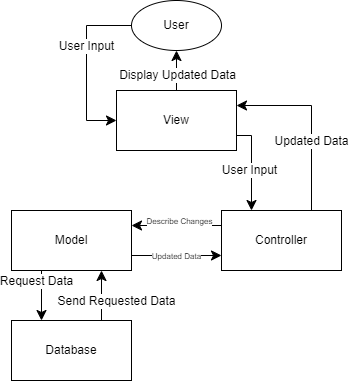
\includegraphics[width = 0.3\textwidth
    ]{images/MVC1.png}
    \caption{Arsitektur MVC}
    \label{fig:enter-label}
\end{figure}

MVC digunakan untuk membagi sebuah aplikasi menjadi tiga bagian, yaitu Model, View, dan Controller \cite{qureshi2014comparison}. Model digunakan untuk pemrosesan data dan hubungan dengan database. Model memberikan data kepada View melalui Controller tanpa mempertimbangkan bagaimana data tersebut dipresentasikan. Bila menerima sebuah notifikasi perubahan atau terjadi sebuah input dari pengguna, Model akan memberi View data yang lebih baru untuk ditampilkan. Tugas Controller adalah untuk menampilkan view berdasarkan input pengguna. Controller menghubungkan Model dengan View. Sebuah input atau pergerakan pada lapisan View akan ditangkap dan diberitakan kepada Controller. Controller akan berinteraksi dengan Model untuk mendapatkan data yang telah diperbaharui dan meneruskan data tersebut pada View. Tugas View adalah untuk menampilkan data tanpa mementingkan proses lain seperti koneksi kepada database. View mempresentasikan data dalam bentuk yang telah diformat dan dapat dibaca oleh pengguna.

MVC berguna untuk sistem yang interaktif, karena memiliki sifat partition-independent, yang berarti bahwa komponen utama dalam MVC dapat beroperasi secara independen satu sama lain, tanpa ada ketergantungan yang kuat di antara mereka. Ini memungkinkan pengembang untuk membuat perubahan tanpa harus khawatir tentang efeknya terhadap komponen yang lain.

MVC, walau bersifat partition-independent, mengalami kesulitan dalam menjalankan proses yang menyebar lapisan pada lokasi yang berbeda, contohnya dengan web application. Pada web application, lapisan View akan berada di device pengguna, namun Controller dan Model bertetap pada server, yang mengakibatkan munculnya permasalahan location-dependant \cite{leff2001web}. Komunikasi pada jaringan, pengiriman data, dan permasalahan dalam sinkronisasi membuat implementasi MVC pada aplikasi berbasis web lebih sulit.


\subsection{MVI}
Arsitektur  MVI,  merupakan  sebuah  arsitektur  yang  menerapkan  aliran  data  searah (unidirectional flow). Model adalah keadaan sebuah aplikasi, yang masih dalam bentuk sebuah data mentah. View adalah representasi keadaan sebuah aplikasi (dari model) yang ditampilkan kepada  pengguna.  Intent  adalah  sebuah  tindakan  yang  dilakukan  sistem  untuk  merespon masukan dari pengguna  dan  perubahan  pada  keadaan  aplikasi  (dari  model). 

\begin{figure}[h]
    \centering
    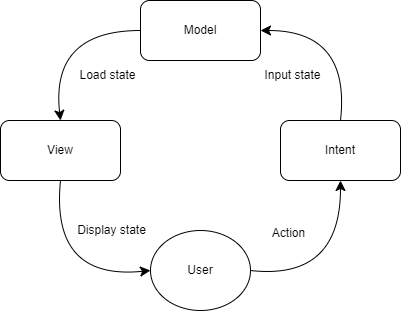
\includegraphics[width = 0.4\textwidth]{images/MVI1.png}
    \caption{Arsitektur MVI}
    \label{fig:enter-label}
\end{figure}

Model-View-Intent, atau MVI, menawarkan banyak kelebihan dan kekurangan dalam pengembangan perangkat lunak perangkat. Salah satu fitur utamanya adalah pemisahan yang jelas antara Model, View, dan Intent, yang membuat kode lebih terstruktur dan lebih mudah digunakan. Dengan aliran data searah, MVI mengurangi risiko bug terkait perubahan tak terduga dan memungkinkan penggunaan status persisten dan berkelanjutan. Selain itu, pendekatan ini memanfaatkan penggunaan logika aplikasi yang stabil, tidak dapat diubah, dan mudah dipahami, sehingga meningkatkan kinerja dan kualitas perangkat lunak. Namun pengguna MVI juga memiliki beberapa kelemahan. Penerapannya seringkali rumit, terutama untuk proyek berukuran kecil atau menengah, dan dapat menimbulkan biaya overhead jika tidak digunakan dengan jujur. Selain itu, terbatasnya ketersediaan sumber daya dan dokumentasi ditambah dengan sifat pendidikan yang berbelit-belit dapat menjadi kendala bagi peserta didik yang belum bias terhadap pendidikan.


\setcounter{subsubsection}{0}
\section{Metodologi}
\subsection{Perancangan}
Bagian ini akan menjelaskan tentang class diagram dan sequence diagram yang menggambarkan implementasi pola arsitektur MVC dan MVI dalam sebuah aplikasi. Diagram ini memberikan visualisasi yang jelas tentang bagaimana kelas-kelas dalam aplikasi berinteraksi satu sama lain untuk mencapai tujuan fungsionalitas tertentu.

\begin{figure}[h]
    \centering
    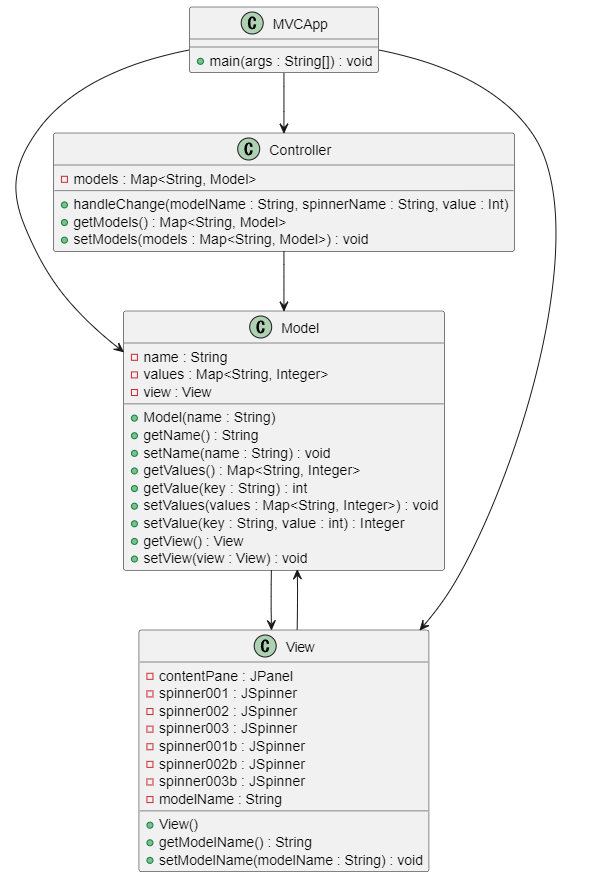
\includegraphics[width=0.6\linewidth]{MVCClassDiagram.png}
    \caption{MVC Class Diagram}
    \label{fig:enter-label}
\end{figure}

\subsubsection{MVCApp}
MVCApp berfungsi sebagai titik masuk utama aplikasi. Kelas ini bertanggung jawab untuk menjalankan aplikasi. \verb |main(args:String[]):void| merupakan metode utama yang menjalankan aplikasi. \\

\subsubsection{Controller}
Controller mengelola interaksi antara model dan view. Kelas ini menerima input dari view dan memperbarui model sesuai dengan input tersebut. 
\paragraph{Atribut}
\verb |models:Map<String,Model>| menyimpan referensi ke model yang digunakan dalam aplikasi. 
\paragraph{Medode}
\begin{itemize}
\item \verb |handleChange(modelName:String,| \verb |spinnerName:String, value:Int):void| mengelola perubahan yang terjadi pada view dan memperbarui model yang sesuai.
\item \verb |getModels():Map<String, Model>| untuk mengembalikan daftar model yang ada. 
\item \verb |setModels(models:Map<String, Model>)| \verb |:void| untuk menyetel model yang digunakan dalam aplikasi. \\
\end{itemize} 

\subsubsection{Model}
Model menyimpan data dan logika bisnis aplikasi. Kelas ini memperbarui data berdasarkan input yang diterima dari controller. 
\paragraph{Atribut} 
\begin{itemize}
\item \verb |name: String| merupakan nama model. 
\item \verb |values: Map<String, Integer>| merupakan data yang disimpan dalam model. 
\item \verb |view: View| merupakan referensi ke view yang menampilkan data dari model ini, memungkinkan model untuk memperbarui tampilan jika ada perubahan data. 
\paragraph{Metode} 
\item \verb |Model(name: String)| merupakan konstruktor untuk membuat model baru dengan nama yang diberikan.
\item \verb |getName() : String| untuk mengembalikan nama model. 
\item \verb |setName(name: String) : void| untuk menyetel model yang digunakan dalam aplikasinama model.
\item \verb |getValues() : Map<String, Integer>| untuk mengembalikan data yang disimpan dalam model. 
\item \verb |setValues(values: Map<String, Integer>)| \verb |:void| untuk menyetel data dalam model.
\item \verb |setValue(key: String, value: int)| \verb |:void| untuk menyetel nilai tertentu berdasarkan kunci yang diberikan.
\item \verb |getView() : View| untuk mengembalikan view yang terkait dengan model.
\item \verb |setView(view: View) : void| untuk menyetel view yang terkait dengan model.
\end{itemize}

\subsubsection{View}
View menampilkan data kepada pengguna dan mengambil input dari pengguna untuk diteruskan ke controller. 
\paragraph{Atribut} 
\begin{itemize}
\item \verb |contentPane: JPanel| merupakan panel utama yang berisi komponen UI.
\item \verb |spinner001, spinner002, spinner003:| \verb |JSpinner:| merupakan spinner untuk input pengguna.
\item \verb |spinner001b, spinner002b, spinner003b:| \verb |JSpinner| merupakan spinner lain untuk input pengguna.
\item \verb |modelName: String| merupakan nama model yang terkait dengan view ini. 
\end{itemize}
\paragraph{Metode} 
\begin{itemize}
\item \verb |View()| merupakan konstruktor untuk membuat view baru.
\item \verb |getModelName() : String| untuk mengembalikan nama model. 
\item \verb |setName(name: String) : void| untuk mengembalikan nama model yang terkait dengan view.
\item \verb |setModelName(modelName: String) : void| untuk menyetel nama model yang terkait dengan view.\\
\end{itemize}

Sequence Diagram adalah alat penting yang digunakan untuk memvisualisasikan interaksi antara berbagai komponen sistem dalam urutan kronologis. Bagian ini akan menjelaskan Sequence Diagram yang menggambarkan proses interaksi antara pengguna, View, Controller, dan Model dalam konteks pola arsitektur Model-View-Controller (MVC). Sequence diagram berikut menjelaskan langkah-langkah proses dari perubahan nilai pada spinner/textbox input hingga nilai balikan ditampilkan oleh spinner/textbox output:

\begin{figure}[h]
    \centering
    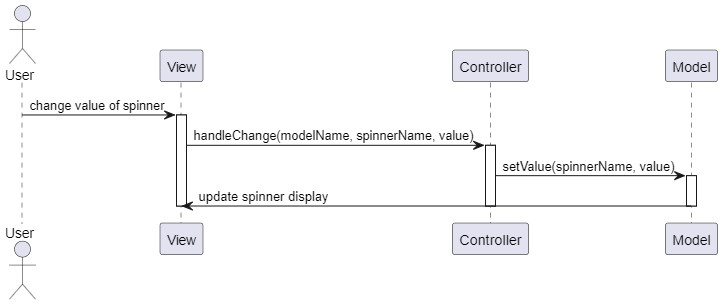
\includegraphics[width=0.8\linewidth]{image.png}
    \caption{MVC Sequence Diagram}
    \label{fig:enter-label}
\end{figure}

\begin{enumerate}
    \item Pengguna mengubah nilai pada spinner atau textbox input di dalam view.
    \item View menangkap perubahan tersebut dan memanggil metode \verb |handleChange(modelName, spinnerName,| \verb |value)| pada controller dengan parameter modelName, spinnerName, dan value.
    \item Controller menerima panggilan dan memanggil metode \verb |setValue(spinnerName,value)| pada model yang sesuai dengan modelName, memperbarui nilai yang terkait dengan spinnerName.
    \item Model memperbarui data internal dan memberitahu view untuk memperbarui tampilan dengan nilai terbaru.
    \item View mengambil nilai terbaru dari model dan menampilkan nilai yang diperbarui kepada pengguna.\\ 
\end{enumerate}

\begin{figure}[h!]
    \centering
    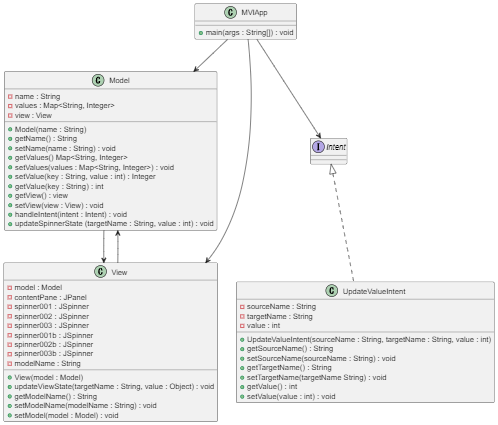
\includegraphics[width=0.7\linewidth]{MVIClassDiagram.png}
    \caption{MVI Class Diagram}
    \label{fig:enter-label}
\end{figure}

\setcounter{subsubsection}{0}

\subsubsection{Model}
Kelas Model bertanggung jawab untuk menyimpan dan mengelola data aplikasi
\paragraph{Atribut}
\verb |name : String| adalah nama model.
\verb |values : Map<String, Integer>| adalah peta nilai yang diidentifikasi dengan kunci string.
\verb |view: View| merupakan referensi ke kelas 'view'.
\paragraph{Metode}
\begin{itemize}
\item \verb |getName()| untuk mengembalikan nama model.
\item \verb |setName(String name)| untuk mengatur nama model.
\item \verb |getValues()|untuk mengembalikan peta nilai.
\item \verb |setValues(Map<String, Integer> values)| mengatur peta nilai.
\item \verb |getValue(String key)| untuk mengembalikan nilai untuk kunci yang diberikan.
\item \verb |setValue(String key, int value)| untuk mengatur nilai untuk kunci yang diberikan.
\item \verb |updateSpinnerState(String targetName,| \verb |int value)| untuk memperbarui status spinner berdasarkan nama target dan nilai yang diberikan.
\item \verb |handleIntent(Intent i)| mengolah intent yang diterima.
\item \verb |getView()| untuk mengembalikan referensi ke objek 'View'.
\item \verb |setView(View view)| untuk mengatur referensi ke objek 'View'.\\
\end{itemize} 

\subsubsection{View}
Kelas View bertanggung jawab untuk menampilkan data kepada pengguna dan memperbarui tampilan berdasarkan perubahan data dalam model.
\paragraph{Atribut} 
\begin{itemize}
\item \verb |contentPane: JPanel| merupakan panel utama yang berisi komponen UI.
\item \verb |spinner001, spinner002, spinner003:| \verb |JSpinner:| merupakan spinner untuk input pengguna.
\item \verb |model: Model| merupakan referensi ke kelas 'Model'.
\end{itemize}
\paragraph{Metode} 
\begin{itemize}
\item \verb |updateViewState(String name, Object| \verb | value)| untuk memperbarui status tampilan berdasarkan nama dan nilai yang diberikan.
\item \verb |getModelName()| untuk mengembalikan nama model. 
\item \verb |setModelName(String name)| untuk mengatur nama model terkait.
\item \verb |getModel()| untuk mengembalikan referensi ke objek 'Model'.
\item \verb |setModel(Model model)| untuk mengatur referensi ke objek 'Model'.\\
\end{itemize}

\subsubsection{MVIApp}
Kelas MVIApp adalah titik awal dari aplikasi. Kelas ini bertanggung jawab untuk memulai aplikasi dan menginisialisasi objek model dan view. Metode utamanya adalah \verb |main(String[] args| yang digunakan untuk menjalankan aplikasi.\\

\subsubsection{Intent}
Kelas Intent adalah abstraksi yang digunakan untuk mewakili tindakan yang harus dilakukan oleh aplikasi. \\

\subsubsection{UpdateValueIntent}
Kelas UpdateValueIntent merupakan subclass dari Intent yang secara khusus digunakan untuk mengatur nilai baru pada model berdasarkan perubahan yang dilakukan pengguna.
\paragraph{Atribut} 
\begin{itemize}
\item \verb |sourceName: String| merupakan nama sumber data yang memicu intent.
\item \verb |targetName:String| merupakan nama target data yang akan diperbarui.
\item \verb |value:int| merupakan nilai baru yang akan diatur.
\end{itemize}
\paragraph{Metode} 
\begin{itemize}
\item \verb |UpdateValueIntent(String sourceName,| \verb |String targetName, int value)| merupakan konstruktor untuk membuat objek intent dengan sumber, target, dan nilai tertentu.
\item \verb |getSourceName()| untuk mengembalikan nama sumber. 
\item \verb |setSourceName(String sourceName)| untuk mengatur nama sumber.
\item \verb |getTargetName()| untuk mengembalikan nama target.
\item \verb |setTargetName(String targetName)| untuk mengatur nama target.
\item \verb |getValue()| untuk mengembalikan nilai intent.
\item \verb |setValue(int value)| untuk mengatur nilai intent. \\
\end{itemize}

\begin{figure}[h]
    \centering
    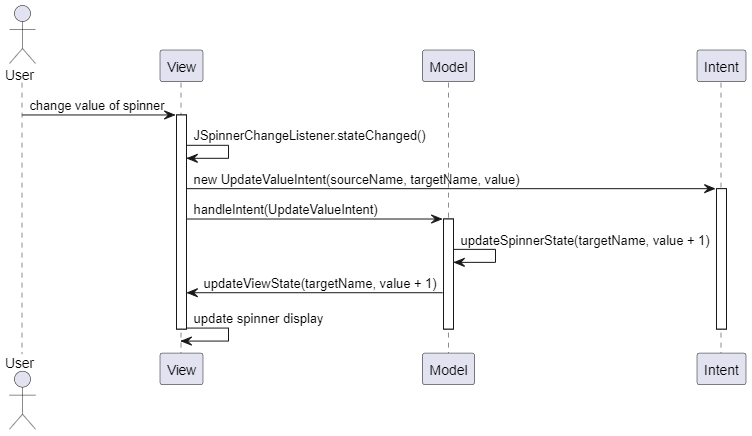
\includegraphics[width=0.8\linewidth]{MVISequence.png}
    \caption{MVI Sequence Diagram}
    \label{fig:enter-label}
\end{figure}

\begin{enumerate}
    \item Pengguna mengubah nilai pada spinner atau textbox input di dalam view.
    \item Listener di view mendeteksi perubahan nilai spinner. Listener ini bertugas untuk menangani perubahan yang terjadi pada komponen UI seperti spinner.
    \item Listener kemudian membuat sebuah instance dari UpdateValueIntent. Intent ini membawa informasi tentang perubahan yang terjadi, termasuk nama sumber, nama target, dan nilai baru.
    \item Intent yang dibuat dikirim ke model melalui metode \verb |handleIntent|. Model bertanggung jawab untuk memproses intent ini dan melakukan tindakan yang sesuai.
    \item Di dalam \verb |handleIntent|, model memanggil metode \verb |updateSpinnerState| dengan target name dan nilai baru yang telah diubah. Dalam contoh ini, nilai baru ditambahkan dengan 1 (value + 1) sebelum diteruskan.
    \item Setelah model memperbarui statusnya, model kemudian memanggil metode di view untuk memperbarui tampilan berdasarkan perubahan ini. Metode \verb |updateViewState| di view dipanggil dengan target name dan nilai baru yang telah ditambahkan dengan 1.
    \item Akhirnya, view memperbarui tampilan spinner untuk mencerminkan nilai baru yang telah diproses. Spinner sekarang menampilkan nilai yang sesuai dengan perubahan yang dilakukan oleh user.\\
\end{enumerate}

\subsection{Implementasi}
Berdasarkan MVC dan MVI di bagian Perancangan, kelas-kelas akan dibuat sesuai dengan arsitektur yang dibahas. MVC, akan memuat tiga kelas, yaitu Model, View, dan Controller, dan satu kelas main, MVCApp. Untuk MVI, Model, View, dan Intent juga akan dibuat bersama dengan kelas main, MVIApp. Satu kelas tambahan akan dibuat untuk MVI, yaitu kelas UpdateValueIntent karena Intent bekerja sebagai interface dan bukan kelas tersendiri. Implementasi akan dibagi ke dalam dua folder. Folder pertama berisi kelas-kelas dan folder kedua berisi tes itu sendiri.
\subsubsection{Model View Intent}
Pada MVI, folder pertama akan dinamakan mvi dan folder kedua test.mvc. File pertama di folder mvi, Intent, diimplementasi oleh UpdateValueIntent dan mengenkapsulasi informasi yang dibutuhkan untuk dilakukannya perubahan, serta menentukan nilai baru untuk target. File Model bertindak sebagai data layer dan state management. Model menyimpan data dalam pasangan kunci-nilai dan melalui metode handleIntent, Model menerima Intent dan mengupdate state. View menangani antarmuka pengguna grafis dari aplikasi. View bertanggung jawab untuk memproses perubahan keadaan di Model. View mengandung beberapa komponen JSpinner yang akan digunakan untuk pengujian. MVIApp adalah kelas utama dan akan menginisialisasi aplikasi dengan mengatur komponen Model dan View, membuat view window menjadi terlihat.
\subsubsection{Model View Controller}
File pertama dari folder mvc, Controller, berfungsi sebagai perantara antara Model dan View. Ini mengatur aliran data dari Model dan pada Model, dan memperbarui View setiap kali terdapat perubahan data. Setiap kali terjadi perubahan nilai, metode handleCange dipanggil. Metode ini memperbarui Model dengan nilai baru dan memicu pembaruan di View. Model berfungsi sebagai data layer dan menyimpan data dalam pasangan key-value pairs melalui HashMap. Model juga memungkinkan perubahan pada View seperti yang terlihat dalam metode setValue. Kelas View bertanggung jawab untuk menampilkan antarmuka pengguna dan menampilkan perubahan status. View mendenga perubahan dari komponen UI dan menyampaikannya pada Controller yang memperbarui Model dan View itu sendiri. View mengextend JFrame dan menggunakan komponen seperti JSpinner, yang akan digunakan untuk dalam pengujian. Metode main MVCApp menginisialisasi Model dan View serta menghubungkan keduanya. Ini memastikan bahwa ketika aplikasi dimulai, View terlihat dan siap untuk berinteraksi.

Penelitian ini dirancang untuk mengukur kinerja aplikasi berbasis dua arsitektur perangkat lunak popular yaitu Model-View-Intent (MVI) dan Model-View-Controller (MVC). Fokus utama pengujian adalah pada dua aspek utama yaitu waktu eksekusi, yang mengukur waktu yang dibutuhkan untuk memproses perubahan pada komponen GUI (JSpinner), dan penggunaan memori, yang mengukur jumlah memori yang digunakan selama proses perubahan komponen. Kode menginisialisasi sejumlah "view" dan "spinner" dalam berbagai kategori, yaitu 1, 25, 50, 75, dan 100.

Pada setiap iterasi pengujian, program membuat model dan view, menghubungkan input dan output spinner, serta mencatat waktu dan memori yang digunakan saat spinner berubah. Hasil pengukuran kemudian disimpan ke dalam file CSV dan ditampilkan di konsol. Proses ini dilakukan dalam dua belas iterasi untuk mendapatkan data yang konsisten dan akurat. Kode MVI dan MVC diimplementasikan dengan inisialisasi dan persiapan yang mirip, namun berbeda dalam cara pengelolaan logika perubahan.
Perbedaan utama antara kedua pendekatan ini adalah bahwa MVI menggunakan pengontrol internal dalam model dan view, yang mengintegrasikan perubahan langsung pada komponen GUI, sedangkan MVC memisahkan logika pengontrol ke dalam kelas yang terpisah, sehingga model dan view berinteraksi melalui controller sebagai mediator. Dalam MVI, logika perubahan lebih terfokus pada intent dan reaksi langsung pada model dan view, sementara dalam MVC, controller berfungsi sebagai penghubung yang mengatur interaksi antara model dan view.

Tujuan pengujian adalah untuk menentukan performa dan efisiensi kedua arsitektur dengan beban kerja yang berbeda. Hasil dari pengukuran performa ini memberikan gambaran tentang seberapa efisien dan efektif masing-masing arsitektur dalam menangani perubahan pada GUI dengan beban kerja yang bervariasi. Data yang terkumpul akan membantu dalam memahami latensi waktu yang dihasilkan oleh masing-masing arsitektur, menilai penggunaan memori dan efisiensi pengelolaan sumber daya, serta membandingkan skala performa dari kedua arsitektur untuk pengambilan keputusan di masa depan. Dengan demikian, pengembang dapat memilih arsitektur yang paling sesuai berdasarkan kebutuhan aplikasi mereka.

\section{Hasil dan Pembahasan}

\subsection{Hasil dan Pembahasan}
Dalam analisis perbandingan antara arsitektur MVC (Model-View-Controller) dan MVI (Model-View-Intent), beberapa temuan kunci diperoleh dari hasil pengujian dan observasi.

\subsubsection{MVC (Model-View-Controller)}
\textbf{Kelebihan:}
\begin{itemize}
    \item Modularitas dan struktur yang jelas memudahkan pengembangan dan pemeliharaan.
    \item Cocok untuk aplikasi dengan kompleksitas rendah hingga menengah.
    \item Waktu eksekusi cepat, dengan total 10 menit dalam pengujian.
\end{itemize}

\textbf{Kekurangan:}
\begin{itemize}
    \item Kesulitan dalam menangani sinkronisasi data yang kompleks.
    \item Potensi peningkatan kompleksitas seiring dengan pertumbuhan aplikasi.
    \item Memerlukan peningkatan beban kerja dalam memastikan sinkronisasi yang tepat antara model, view, dan controller.
\end{itemize}

\subsubsection{MVI (Model-View-Intent)}
\textbf{Kelebihan:}
\begin{itemize}
    \item Efisiensi dan skalabilitas yang lebih baik, terutama dalam aplikasi yang sangat reaktif.
    \item Manajemen status yang lebih mudah dilacak, mengurangi risiko kesalahan pengelolaan status.
    \item Cocok untuk aplikasi dengan kebutuhan responsivitas tinggi dan perubahan status yang sering.
\end{itemize}

\textbf{Kekurangan:}
\begin{itemize}
    \item Waktu eksekusi lebih lambat dibandingkan MVC, dengan total 16 menit dalam pengujian.
    \item Memerlukan pemahaman yang lebih dalam tentang aliran data searah dan konsep immutable state.
\end{itemize}

\subsection{Analisis Perbandingan}
Dari hasil pengujian dan pembandingan, dapat ditarik beberapa kesimpulan:

1. \textbf{Kecepatan Eksekusi:} MVC memiliki keunggulan dalam hal waktu eksekusi yang lebih cepat, cocok untuk aplikasi dengan kebutuhan respon cepat. Sementara MVI lebih lambat namun lebih baik dalam manajemen status yang kompleks.

2. \textbf{Manajemen Status:} MVI memiliki keunggulan dalam manajemen status yang lebih baik, mengurangi risiko kesalahan dan memudahkan penelusuran bug.

3. \textbf{Skalabilitas:} MVI menawarkan skalabilitas yang lebih baik dalam mengelola perubahan status yang sering, cocok untuk aplikasi dengan kebutuhan responsivitas tinggi.

4. \textbf{Kesulitan Pengembangan:} MVC cenderung lebih mudah dipahami bagi pengembang baru, sementara MVI memerlukan pemahaman yang lebih dalam tentang konsep immutable state.

% \subsection{Perancangan dan Implementasi}\label{AA}
% Bagian ini akan menjelaskan tentang class diagram dan sequence diagram yang menggambarkan implementasi pola arsitektur MVC dan MVI dalam sebuah aplikasi. Diagram ini memberikan visualisasi yang jelas tentang bagaimana kelas-kelas dalam aplikasi berinteraksi satu sama lain untuk mencapai tujuan fungsionalitas tertentu.

% \begin{figure}[h]
%     \centering
%     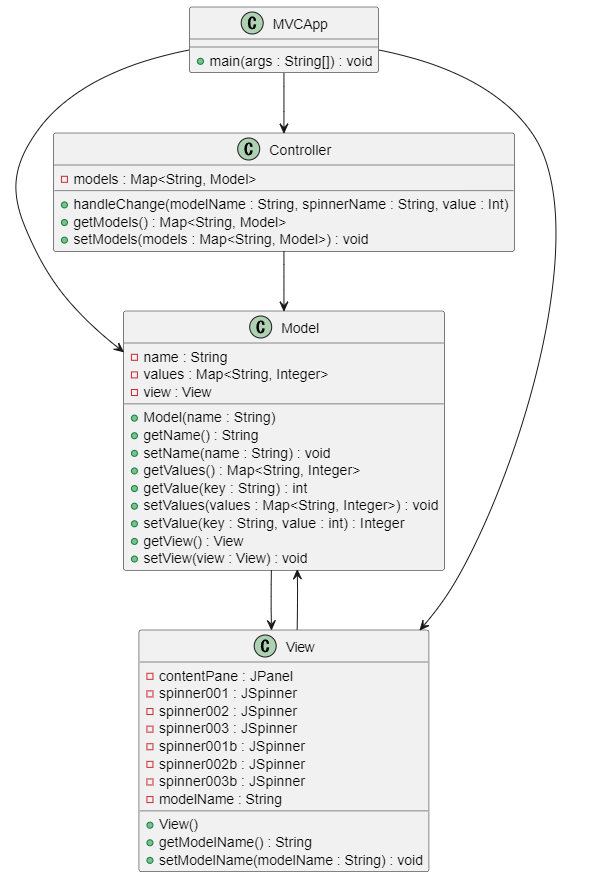
\includegraphics[width=0.6\linewidth]{MVCClassDiagram.png}
%     \caption{MVC Class Diagram}
%     \label{fig:enter-label}
% \end{figure}

% \subsubsection{MVCApp}
% MVCApp berfungsi sebagai titik masuk utama aplikasi. Kelas ini bertanggung jawab untuk menjalankan aplikasi. \verb |main(args:String[]):void| merupakan metode utama yang menjalankan aplikasi. \\

% \subsubsection{Controller}
% Controller mengelola interaksi antara model dan view. Kelas ini menerima input dari view dan memperbarui model sesuai dengan input tersebut. 
% \paragraph{Atribut}
% \verb |models:Map<String,Model>| menyimpan referensi ke model yang digunakan dalam aplikasi. 
% \paragraph{Medode}
% \begin{itemize}
% \item \verb |handleChange(modelName:String,| \verb |spinnerName:String, value:Int):void| mengelola perubahan yang terjadi pada view dan memperbarui model yang sesuai.
% \item \verb |getModels():Map<String, Model>| untuk mengembalikan daftar model yang ada. 
% \item \verb |setModels(models:Map<String, Model>)| \verb |:void| untuk menyetel model yang digunakan dalam aplikasi. \\
% \end{itemize} 

% \subsubsection{Model}
% Model menyimpan data dan logika bisnis aplikasi. Kelas ini memperbarui data berdasarkan input yang diterima dari controller. 
% \paragraph{Atribut} 
% \begin{itemize}
% \item \verb |name: String| merupakan nama model. 
% \item \verb |values: Map<String, Integer>| merupakan data yang disimpan dalam model. 
% \item \verb |view: View| merupakan referensi ke view yang menampilkan data dari model ini, memungkinkan model untuk memperbarui tampilan jika ada perubahan data. 
% \paragraph{Metode} 
% \item \verb |Model(name: String)| merupakan konstruktor untuk membuat model baru dengan nama yang diberikan.
% \item \verb |getName() : String| untuk mengembalikan nama model. 
% \item \verb |setName(name: String) : void| untuk menyetel model yang digunakan dalam aplikasinama model.
% \item \verb |getValues() : Map<String, Integer>| untuk mengembalikan data yang disimpan dalam model. 
% \item \verb |setValues(values: Map<String, Integer>)| \verb |:void| untuk menyetel data dalam model.
% \item \verb |setValue(key: String, value: int)| \verb |:void| untuk menyetel nilai tertentu berdasarkan kunci yang diberikan.
% \item \verb |getView() : View| untuk mengembalikan view yang terkait dengan model.
% \item \verb |setView(view: View) : void| untuk menyetel view yang terkait dengan model.
% \end{itemize}

% \subsubsection{View}
% View menampilkan data kepada pengguna dan mengambil input dari pengguna untuk diteruskan ke controller. 
% \paragraph{Atribut} 
% \begin{itemize}
% \item \verb |contentPane: JPanel| merupakan panel utama yang berisi komponen UI.
% \item \verb |spinner001, spinner002, spinner003:| \verb |JSpinner:| merupakan spinner untuk input pengguna.
% \item \verb |spinner001b, spinner002b, spinner003b:| \verb |JSpinner| merupakan spinner lain untuk input pengguna.
% \item \verb |modelName: String| merupakan nama model yang terkait dengan view ini. 
% \end{itemize}
% \paragraph{Metode} 
% \begin{itemize}
% \item \verb |View()| merupakan konstruktor untuk membuat view baru.
% \item \verb |getModelName() : String| untuk mengembalikan nama model. 
% \item \verb |setName(name: String) : void| untuk mengembalikan nama model yang terkait dengan view.
% \item \verb |setModelName(modelName: String) : void| untuk menyetel nama model yang terkait dengan view.\\
% \end{itemize}

% Sequence Diagram adalah alat penting yang digunakan untuk memvisualisasikan interaksi antara berbagai komponen sistem dalam urutan kronologis. Bagian ini akan menjelaskan Sequence Diagram yang menggambarkan proses interaksi antara pengguna, View, Controller, dan Model dalam konteks pola arsitektur Model-View-Controller (MVC). Sequence diagram berikut menjelaskan langkah-langkah proses dari perubahan nilai pada spinner/textbox input hingga nilai balikan ditampilkan oleh spinner/textbox output:

% \begin{figure}[h]
%     \centering
%     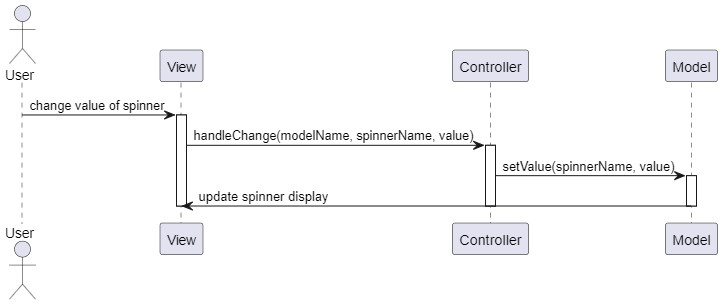
\includegraphics[width=0.8\linewidth]{image.png}
%     \caption{MVC Sequence Diagram}
%     \label{fig:enter-label}
% \end{figure}

% \begin{enumerate}
%     \item Pengguna mengubah nilai pada spinner atau textbox input di dalam view.
%     \item View menangkap perubahan tersebut dan memanggil metode \verb |handleChange(modelName, spinnerName,| \verb |value)| pada controller dengan parameter modelName, spinnerName, dan value.
%     \item Controller menerima panggilan dan memanggil metode \verb |setValue(spinnerName,value)| pada model yang sesuai dengan modelName, memperbarui nilai yang terkait dengan spinnerName.
%     \item Model memperbarui data internal dan memberitahu view untuk memperbarui tampilan dengan nilai terbaru.
%     \item View mengambil nilai terbaru dari model dan menampilkan nilai yang diperbarui kepada pengguna.\\ 
% \end{enumerate}
% \vspace{5cm} %this might mess up pages once its complete
% \begin{figure}[h!]
%     \centering
%     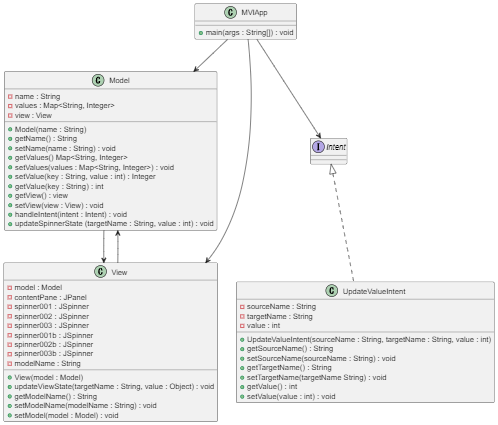
\includegraphics[width=0.7\linewidth]{MVIClassDiagram.png}
%     \caption{MVI Class Diagram}
%     \label{fig:enter-label}
% \end{figure}

% \setcounter{subsubsection}{0}

% \subsubsection{Model}
% Kelas Model bertanggung jawab untuk menyimpan dan mengelola data aplikasi
% \paragraph{Atribut}
% \verb |name : String| adalah nama model.
% \verb |values : Map<String, Integer>| adalah peta nilai yang diidentifikasi dengan kunci string.
% \verb |view: View| merupakan referensi ke kelas 'view'.
% \paragraph{Metode}
% \begin{itemize}
% \item \verb |getName()| untuk mengembalikan nama model.
% \item \verb |setName(String name)| untuk mengatur nama model.
% \item \verb |getValues()|untuk mengembalikan peta nilai.
% \item \verb |setValues(Map<String, Integer> values)| mengatur peta nilai.
% \item \verb |getValue(String key)| untuk mengembalikan nilai untuk kunci yang diberikan.
% \item \verb |setValue(String key, int value)| untuk mengatur nilai untuk kunci yang diberikan.
% \item \verb |updateSpinnerState(String targetName,| \verb |int value)| untuk memperbarui status spinner berdasarkan nama target dan nilai yang diberikan.
% \item \verb |handleIntent(Intent i)| mengolah intent yang diterima.
% \item \verb |getView()| untuk mengembalikan referensi ke objek 'View'.
% \item \verb |setView(View view)| untuk mengatur referensi ke objek 'View'.\\
% \end{itemize} 

% \subsubsection{View}
% Kelas View bertanggung jawab untuk menampilkan data kepada pengguna dan memperbarui tampilan berdasarkan perubahan data dalam model.
% \paragraph{Atribut} 
% \begin{itemize}
% \item \verb |contentPane: JPanel| merupakan panel utama yang berisi komponen UI.
% \item \verb |spinner001, spinner002, spinner003:| \verb |JSpinner:| merupakan spinner untuk input pengguna.
% \item \verb |model: Model| merupakan referensi ke kelas 'Model'.
% \end{itemize}
% \paragraph{Metode} 
% \begin{itemize}
% \item \verb |updateViewState(String name, Object| \verb | value)| untuk memperbarui status tampilan berdasarkan nama dan nilai yang diberikan.
% \item \verb |getModelName()| untuk mengembalikan nama model. 
% \item \verb |setModelName(String name)| untuk mengatur nama model terkait.
% \item \verb |getModel()| untuk mengembalikan referensi ke objek 'Model'.
% \item \verb |setModel(Model model)| untuk mengatur referensi ke objek 'Model'.\\
% \end{itemize}

% \subsubsection{MVIApp}
% Kelas MVIApp adalah titik awal dari aplikasi. Kelas ini bertanggung jawab untuk memulai aplikasi dan menginisialisasi objek model dan view. Metode utamanya adalah \verb |main(String[] args| yang digunakan untuk menjalankan aplikasi.\\

% \subsubsection{Intent}
% Kelas Intent adalah abstraksi yang digunakan untuk mewakili tindakan yang harus dilakukan oleh aplikasi. \\

% \subsubsection{UpdateValueIntent}
% Kelas UpdateValueIntent merupakan subclass dari Intent yang secara khusus digunakan untuk mengatur nilai baru pada model berdasarkan perubahan yang dilakukan pengguna.
% \paragraph{Atribut} 
% \begin{itemize}
% \item \verb |sourceName: String| merupakan nama sumber data yang memicu intent.
% \item \verb |targetName:String| merupakan nama target data yang akan diperbarui.
% \item \verb |value:int| merupakan nilai baru yang akan diatur.
% \end{itemize}
% \paragraph{Metode} 
% \begin{itemize}
% \item \verb |UpdateValueIntent(String sourceName,| \verb |String targetName, int value)| merupakan konstruktor untuk membuat objek intent dengan sumber, target, dan nilai tertentu.
% \item \verb |getSourceName()| untuk mengembalikan nama sumber. 
% \item \verb |setSourceName(String sourceName)| untuk mengatur nama sumber.
% \item \verb |getTargetName()| untuk mengembalikan nama target.
% \item \verb |setTargetName(String targetName)| untuk mengatur nama target.
% \item \verb |getValue()| untuk mengembalikan nilai intent.
% \item \verb |setValue(int value)| untuk mengatur nilai intent. \\
% \end{itemize}

% \begin{figure}[h]
%     \centering
%     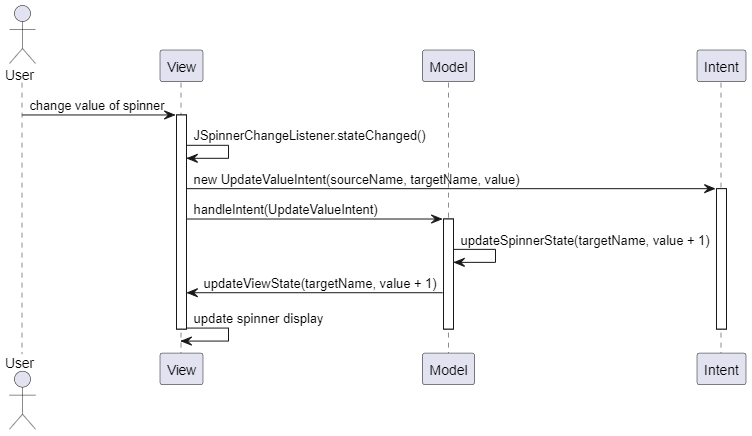
\includegraphics[width=0.8\linewidth]{MVISequence.png}
%     \caption{MVI Sequence Diagram}
%     \label{fig:enter-label}
% \end{figure}

% \begin{enumerate}
%     \item Pengguna mengubah nilai pada spinner atau textbox input di dalam view.
%     \item Listener di view mendeteksi perubahan nilai spinner. Listener ini bertugas untuk menangani perubahan yang terjadi pada komponen UI seperti spinner.
%     \item Listener kemudian membuat sebuah instance dari UpdateValueIntent. Intent ini membawa informasi tentang perubahan yang terjadi, termasuk nama sumber, nama target, dan nilai baru.
%     \item Intent yang dibuat dikirim ke model melalui metode \verb |handleIntent|. Model bertanggung jawab untuk memproses intent ini dan melakukan tindakan yang sesuai.
%     \item Di dalam \verb |handleIntent|, model memanggil metode \verb |updateSpinnerState| dengan target name dan nilai baru yang telah diubah. Dalam contoh ini, nilai baru ditambahkan dengan 1 (value + 1) sebelum diteruskan.
%     \item Setelah model memperbarui statusnya, model kemudian memanggil metode di view untuk memperbarui tampilan berdasarkan perubahan ini. Metode \verb |updateViewState| di view dipanggil dengan target name dan nilai baru yang telah ditambahkan dengan 1.
%     \item Akhirnya, view memperbarui tampilan spinner untuk mencerminkan nilai baru yang telah diproses. Spinner sekarang menampilkan nilai yang sesuai dengan perubahan yang dilakukan oleh user.\\
% \end{enumerate}
\newpage

\section{Kesimpulan}
Dari hasil analisis di atas, dapat disimpulkan bahwa arsitektur Model-View-Controller (MVC) dan Model-View-Intent (MVI) masing-masing memiliki kelebihan dan kekurangan yang khas, yang dapat mempengaruhi keputusan pengembang dalam memilih arsitektur yang paling sesuai untuk proyek mereka.

\subsection{Kelebihan dan Kekurangan MVC}

MVC menawarkan modularitas dan struktur yang jelas, yang sangat berguna dalam pengembangan proyek berskala besar. Pemisahan yang jelas antara Model, View, dan Controller memudahkan pemeliharaan dan pengembangan lebih lanjut. Hal ini juga memungkinkan tim pengembang untuk bekerja secara paralel pada komponen yang berbeda tanpa banyak konflik.

Namun, MVC bisa menjadi sangat kompleks seiring bertambahnya interaksi dan dependensi antar komponen. Sinkronisasi data antara Model dan View melalui Controller sering kali memerlukan banyak sumber daya, terutama pada aplikasi web yang melibatkan banyak komunikasi jaringan. Pengembang harus menangani pembaruan status secara hati-hati untuk menghindari kondisi balapan dan bug lainnya yang bisa sulit dilacak.

\textbf{Rekomendasi:} MVC cocok untuk proyek besar dengan tim pengembang yang terpisah dan memerlukan modularitas yang tinggi. Ini juga ideal untuk aplikasi dengan interaksi pengguna yang tidak terlalu kompleks atau untuk sistem di mana performa jaringan bukanlah kendala utama.

\subsection{Kelebihan dan Kekurangan MVI}

MVI, dengan aliran data searah dan status yang tidak dapat diubah, menawarkan efisiensi dan konsistensi yang lebih baik dalam pengelolaan status aplikasi. Pendekatan ini mengurangi kemungkinan kondisi balapan dan memudahkan debugging karena aliran data yang lebih dapat diprediksi. MVI juga lebih hemat sumber daya karena setiap perubahan status dikelola dengan efisien dan hanya memicu pembaruan yang diperlukan.

Namun, MVI memiliki kurva belajar yang lebih tinggi karena konsep aliran data searah dan manajemen status yang lebih ketat. Implementasi MVI bisa lebih rumit pada awalnya, terutama bagi pengembang yang belum terbiasa dengan pola ini. Selain itu, perubahan kecil dalam UI dapat memerlukan pembaruan yang lebih luas dalam Intent dan Model, yang bisa menjadi kurang efisien dalam beberapa kasus.

\textbf{Rekomendasi:} MVI sangat cocok untuk aplikasi yang sangat reaktif dan berorientasi pada pengguna, di mana konsistensi status dan efisiensi sumber daya sangat penting. Ini juga ideal untuk aplikasi yang dijalankan pada perangkat dengan keterbatasan sumber daya seperti ponsel pintar.

\subsection{Analisis Perbandingan}

Secara keseluruhan, pilihan antara MVC dan MVI sebaiknya disesuaikan dengan kebutuhan spesifik proyek, termasuk ukuran aplikasi, kompleksitas interaksi, dan sumber daya yang tersedia. 

\begin{itemize}
    \item \textbf{Untuk aplikasi skala besar dengan tim pengembang terpisah:} MVC lebih cocok karena modularitas dan struktur yang jelas.
    \item \textbf{Untuk aplikasi dengan kebutuhan daya tanggap tinggi dan sumber daya terbatas:} MVI lebih efisien karena aliran data searah dan status yang tidak dapat diubah.
    \item \textbf{Untuk aplikasi web dengan banyak interaksi jaringan:} MVC mungkin lebih memerlukan optimasi tambahan untuk mengatasi sinkronisasi data yang intensif.
    \item \textbf{Untuk aplikasi seluler dengan kebutuhan efisiensi baterai:} MVI memberikan keuntungan dalam efisiensi penggunaan sumber daya.
\end{itemize}

\subsection{Kesimpulan Akhir}

Pemahaman yang baik tentang karakteristik dan kinerja masing-masing arsitektur akan membantu pengembang dalam membuat keputusan yang tepat untuk proyek mereka. Kedua arsitektur ini, dengan kelebihan dan kekurangannya, memberikan kerangka kerja yang kuat untuk mengembangkan aplikasi yang scalable, maintainable, dan efisien. Pengembang harus mempertimbangkan faktor-faktor seperti kebutuhan spesifik aplikasi, kemampuan tim, dan tujuan jangka panjang proyek untuk memilih arsitektur yang paling sesuai.
\section*{}
\bibliographystyle{plain}
\bibliography{mybib}

\end{document}
